\documentclass[11pt]{article}

\usepackage[a4paper,margin=0.86in]{geometry}
\usepackage{amsmath,amssymb,amsthm}
\usepackage{graphicx}
\usepackage[hidelinks]{hyperref}
\usepackage{microtype}
\usepackage[compact]{titlesec}
\titlespacing*{\section}{0pt}{1.5ex plus .3ex}{.7ex}

\newtheorem{theorem}{Theorem}
\newtheorem{corollary}{Corollary}
\newcommand{\R}{\mathcal R}
\newcommand{\indL}{\operatorname{ind}_{L}}

\title{The Power Criterion for One-Sided Drazin Invertibility}
\author{Automatic math-discovery run \texttt{fa\_banach\_001}}
\date{August 11, 2026}

\begin{document}
\maketitle

\section*{Source question}

\noindent\textbf{Source:} Kai Yan, \emph{One-sided Drazin inverses in Banach
algebras and perturbations of B-Fredholm spectra}, arXiv:2402.13574 (first
posted February 21, 2024) [1].

Question 2.9 on page 8 asks whether \(a\) is left (respectively right) Drazin
invertible with index \(n\) if and only if \(a^n\) is left (respectively
right) group invertible.

\begin{center}
  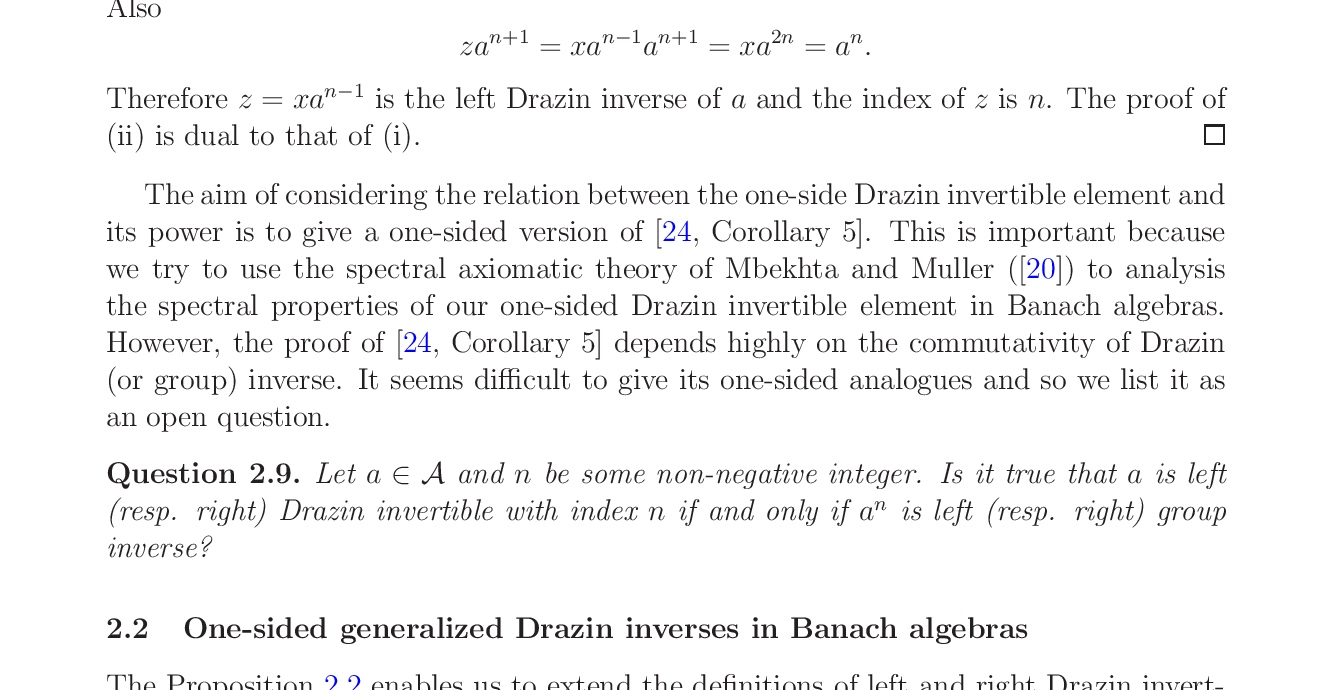
\includegraphics[width=0.96\linewidth]{figures/open_question_crop.jpg}
\end{center}

\section*{Result and convention}

This packet gives a \textbf{candidate full resolution}.  For every positive
integer \(n\), the power condition is equivalent to one-sided Drazin index
\emph{at most} \(n\).  Equivalently, it is equivalent to the existence of a
one-sided Drazin inverse satisfying the defining equations with exponent
\(n\).  The proof is purely algebraic and works in every unital ring.

This distinction resolves two wording issues in the printed question.  If
``index'' means the minimal index---as the author explicitly specifies in a
later paper [2]---then equality with \(n\) is too strong: for
example, \(a=1\) has minimal index zero although \(a^n=1\) is group invertible
for every \(n\geq1\).  Also, the printed allowance \(n=0\) is false in
general because \(a^0=1\) is always group invertible, whereas not every \(a\)
is one-sided invertible (take \(a=0\)).

\section*{Definitions}

Let \(\R\) be a unital ring.  An element \(b\in\R\) is \emph{left group
invertible} if some \(x\in\R\) satisfies
\[
 bxb=xb^2,\qquad x^2b=x,\qquad xb^2=b.
\]
An element \(a\in\R\) admits a \emph{left Drazin inverse with exponent
\(n\)} if some \(z\in\R\) satisfies
\begin{equation}\label{eq:drazin}
 aza=za^2,\qquad z^2a=z,\qquad za^{n+1}=a^n.
\end{equation}
Its minimal possible exponent is denoted \(\indL(a)\).  The right-hand
notions reverse all products in these equations.

\section*{Idea of the proof}

Suppose \(b=a^n\) has a left group inverse \(x\).  The idempotent
\(e=xb\) splits the ring into Peirce corners.  With \(p=1-e\), the element
\(a\) is lower triangular:
\[
 a=\begin{pmatrix}A&0\\ C&D\end{pmatrix},
 \qquad A^n\text{ is left invertible},\qquad D^n=0.
\]
Thus \(A\) itself has a left inverse \(L\).  The finite Sylvester sum
\[
 T=\sum_{k=0}^{n-1}D^kCL^{k+1}
\]
satisfies \(TA-DT=C\).  Since \(T^2=0\), conjugation by \(1+T\) removes the
off-diagonal corner and turns \(a\) into \(A+D\).  The element \(L\), placed
in the \(A\)-corner, is visibly a left Drazin inverse with exponent \(n\).

\section*{Sharp power theorem}

\begin{theorem}\label{thm:main}
Let \(\R\) be a unital ring, let \(a\in\R\), and let \(n\geq1\).  The
following are equivalent:
\begin{enumerate}
\item \(a^n\) is left group invertible;
\item \(a\) admits a left Drazin inverse satisfying
      \eqref{eq:drazin} with exponent \(n\);
\item \(a\) is left Drazin invertible and \(\indL(a)\leq n\).
\end{enumerate}
The analogous three right-handed statements are equivalent.
\end{theorem}

\begin{proof}
We prove the nontrivial implication (1)\(\Rightarrow\)(2).  Put \(b=a^n\),
and let \(x\) be a left group inverse of \(b\).  Its defining equations give
\[
 bxb=b,\qquad x^2b=x,\qquad xb^2=b.
\]
Set \(e=xb\) and \(p=1-e\).  Then
\[
 e^2=x(bxb)=xb=e,\qquad be=b=eb,\qquad bp=pb=0.
\]
The right annihilator of \(b\) is exactly \(p\R\): if \(br=0\), then
\(er=xbr=0\), hence \(r=pr\); the reverse inclusion follows from \(bp=0\).
Since \(a\) commutes with \(b=a^n\), we have
\(b(ap)=a(bp)=0\), and therefore \(ap=pap\), or \(eap=0\).

Define the Peirce corners
\[
 A=eae\in e\R e,\qquad C=pae\in p\R e,\qquad D=pap\in p\R p.
\]
Thus \(a=A+C+D\), with the formal block shape displayed in the proof idea.
Taking powers and using \(bp=pb=0\) gives
\begin{equation}\label{eq:diagdata}
 A^n=ea^ne=b,\qquad D^n=pa^np=0.
\end{equation}
Moreover \(h=exe\) is a left inverse of \(A^n\) in \(e\R e\), since
\[
 hA^n=exe b=exb=e.
\]
Consequently
\[
 L=hA^{n-1}\in e\R e,\qquad LA=e.
\]

Now put
\begin{equation}\label{eq:T}
 T=\sum_{k=0}^{n-1}D^kCL^{k+1}\in p\R e.
\end{equation}
Because \(LA=e\) and \(D^n=0\), the sum telescopes:
\begin{equation}\label{eq:sylvester}
 TA-DT
 =\sum_{k=0}^{n-1}D^kCL^k-
   \sum_{k=1}^{n}D^kCL^k=C.
\end{equation}
Also \(T^2=0\), so \(u=1+T\) is invertible with \(u^{-1}=1-T\).  Direct
Peirce multiplication, using \eqref{eq:sylvester}, yields
\begin{equation}\label{eq:similarity}
 u^{-1}au=A+D.
\end{equation}

In the diagonalized coordinates set \(z'=L\).  Orthogonality of the two
corners, \(LA=e\), and \(D^n=0\) give
\begin{align*}
 (A+D)L(A+D)&=ALA=LA^2,\\
 L^2(A+D)&=L,\\
 L(A+D)^{n+1}&=LA^{n+1}=A^n=(A+D)^n.
\end{align*}
Therefore \(z=uLu^{-1}\) satisfies all three equations
\eqref{eq:drazin} for \(a\), proving (2).

For (2)\(\Rightarrow\)(1), let \(z\) satisfy \eqref{eq:drazin} and put
\(e=za\), \(p=1-e\).  The same elementary identities used in the source's
Proposition 2.7 show that \(p\) commutes with \(a\), \((ap)^n=0\), and the
\(e\)-corner of \(a\) is left invertible.  Hence the \(e\)-corner of \(a^n\)
is left invertible and its \(p\)-corner is zero.  If \(H\) is a left inverse
of that \(e\)-corner, then, extended by zero on the \(p\)-corner,
\[
 (a^n)H(a^n)=H(a^n)^2=a^n,\qquad H^2a^n=H;
\]
so \(H\) is a left group inverse of \(a^n\).

Finally, (2) and (3) are equivalent because an equation
\(za^{k+1}=a^k\) with \(k\leq n\) remains true after right multiplication by
\(a^{n-k}\).  This proves the left-handed result.  Applying it in the
opposite ring \(\R^{\mathrm{op}}\) proves the right-handed result.
\end{proof}

\begin{corollary}[Exact minimal index]
For \(n\geq2\), \(\indL(a)=n\) if and only if \(a^n\) is left group
invertible but \(a^{n-1}\) is not.  For \(n=1\), exact index one means that
\(a\) is left group invertible but not left invertible.  The right-handed
statements are dual.
\end{corollary}

\section*{Machine-checkable audit}

The accompanying exact SymPy script instantiates a nontrivial \(5\times5\)
lower-triangular example with \(n=3\).  It verifies the Sylvester identity,
the similarity \eqref{eq:similarity}, the commuting idempotent, nilpotence of
the bad corner, all three constructed left-Drazin equations, and all three
left-group equations for \(a^n\).  No floating-point computation is used.

\section*{Novelty, limitations, and review recommendation}

A bounded search of the run indexes, exact question wording, core keywords,
and the author's 2025 follow-up [2] found no later source proving
this power criterion.  The follow-up clarifies the minimal-index convention
but studies other fundamental properties.  Novelty confidence is moderate,
pending specialist review.

The result concerns ordinary one-sided Drazin invertibility, not the
generalized Drazin notions later in the source paper.  It strengthens the
ambient category from Banach algebras to unital rings.  Promotion for expert
review is recommended; the main review points are the annihilator identity
\(\operatorname{ann}_r(b)=p\R\) and the finite Sylvester conjugation
\eqref{eq:T}--\eqref{eq:similarity}.

\enlargethispage{2\baselineskip}
\section*{References}
{\small\raggedright
\noindent[1] K. Yan, \emph{One-sided Drazin inverses in Banach algebras and
perturbations of B-Fredholm spectra}, arXiv:2402.13574.\par
\noindent[2] K. Yan, \emph{On the spectral identities and fundamental
properties of one-sided Drazin inverses in Banach algebras},
arXiv:2504.18995.\par}

\end{document}
